\renewcommand{\contentsname}{Indice}
\tableofcontents
% * PARA MODIFICAR ALGÚN TEMA, HAY QUE IR AL ARCHIVO CORRESPONDIENTE, Y SI SE QUIERE AÑADIR ALGÚN SUB APARTADO, SE AÑADE AHÍ *%
\newpage
\section{Introducción}
\setlength{\parindent}{0ex}
\subsection{Movimiento}
En este apartado veremos un repaso de los movimientos más básicos.


\subsubsection{MRU y MRUA}

Partiendo de la \textit{\(2^a\) Ley de Newton}, sabemos que la Fuerza es igual a la masa por su aceleración:
\[\vec{F} = m\vec{a}\]
Podemos descomponer la fuerza en sus componentes horizontales y verticales:
\[
        \vec{F_{x}}=\frac{\partial^{2}\vec{x}}{\partial{t}}m
        \to
        m\frac{\partial^2 \vec{x}}{\partial t} = 0
        \Leftrightarrow
        \frac{\partial^2{\vec{x}}}{\partial{t}} = 0
\]
\[
        \vec{F_{y}}=F_{y}\hat{\jmath}
        \to
        \vec{F_y} = m\frac{\partial\vec{v}}{\partial t}\Leftrightarrow
        \frac{\vec{F_y}}{m} = \vec{a_y}
\]
Es decir, cuando \(\vec{F_x}\) = 0N, \(\vec{a}=0\)m/\(s^2\), por lo que la velocidad es constante, \(\vec{v}=cte\), solo si \(\vec{F_y}\neq 0\)N y \(\vec{a_y} = \vec{a} = \frac{\vec{F_y}}{m}=cte\).\par \vspace{0.5cm} Sabiendo esto y las expresiones de la aceleración y la velocidad, podemos definir las expresiones del \textbf{MRU} y \textbf{MRUA}: \par \vspace{0.5cm} \hspace{5cm}
\( \vec{a} = \frac{\partial \vec{v} }{\partial t}\) Y \( \vec{v} = \frac{\partial \vec{x} }{\partial t}\) \par \vspace{0.5cm} Obtenemos:
\[
        \int_{0}^{t}{\vec{a}\hspace{1mm}\partial{t}} = \int_{0}\partial{t}
        \to
        \boxed{\vec{v} = \vec{v_o} + \vec{a}t}
\]
\[
        \int_{0}^{t}{\vec{v}\hspace{1mm}\partial{t}} = \int_{0}{\partial{\vec{x}}}
        \to
        \boxed{\vec{x} = \vec{x_o} + \vec{v_0}t}
\]
\hspace{1.1cm} Si \( \vec{v} = \vec{v_o} + \vec{a}t\)
y
\( \vec{a} = cte \to\) \fbox{\(\vec{x} = \vec{x_o} + \vec{v_0}t + \frac{\vec{a}t^2}{2}\)}
\vspace{5cm}
\subsubsection{MCU y MCUA}
\hspace{0.5cm}
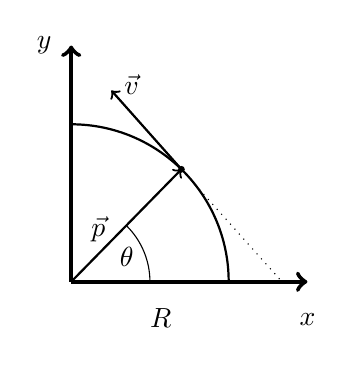
\begin{tikzpicture}[x=1cm,y=1cm]
        \draw[->,ultra thick] (0,0)--(3,0) node[above = -20]{\(x\)} node[above = -13, left = 45] {\(R\)};
        \draw[->,ultra thick] (0,0)--(0,3) node[left = 3]{\(y\)};
        \draw[thick] (2,0) arc (0:90:2);
        \draw[thin] (1,0) arc (0:45:1) node[above = -18]{\( \theta\)};
        \draw[->,thick] (1.4,1.42828) -- (0.5098765432099,2.429629629629) node[above = 2, right = 1]{\(\vec{v}\)};
        \draw[dotted] (1.4,1.42828) -- (2.676296,0);
        \draw[->,thick] (0,0) -- (1.4,1.42828) node[left = 30, above = -30]{\(\vec{p}\)};
        \filldraw[color = black] (1.4,1.42828) circle (1pt);
\end{tikzpicture} \par
El \textbf{MCU} o Movimiento Circular Uniforme, se genera en las rotaciones de un cuerpo respecto a un punto \(p\).
Podemos analizar la posición de un punto cualquiera, en función de las componentes horizontales y verticales:
\[
        \boxed{\vec{P}(t)=(\vec{x}(t),\vec{y}(t))=R(\cos{\theta}\vec{\imath} + \sin{\theta}\vec{\jmath})}
\]
Sabemos que el modulo de \(\vec{P}(t)\) es lo mismo que: \(\left | \vec{P} \right | = R\) y que al derivar un angulo cualquiera en función del tiempo, obtenemos la velocidad angular por unidad de tiempo: \[
        \frac{\partial \theta}{\partial t} = \frac{v}{R}t = wt\
\]
Por lo tanto, podemos concluir con lo siguiente
\[
        \vec{v} =\frac{\partial \vec{P}}{\partial t} =R \hspace{1.35mm} (w\cos{\theta}\vec{\jmath} - w\sin{\theta}\vec{\imath}\hspace{1mm})  = \boxed{Rw \hspace{1.35mm} (\cos{\theta}\vec{\jmath} - \sin{\theta}\vec{\imath}\hspace{1mm})}
\]
Y que el modulo de la velocidad es constante:
\[
        \left | \vec{v} \right | = wR = cte
\]
Evidentemente podemos calcular a partir de la velocidad, el vector aceleración:
\[
        \vec{a} =\frac{\partial \vec{v}}{\partial t} = -Rw^2 \hspace{1.35mm}(\cos{\theta}\vec{\imath} + \sin{\theta}\vec{\jmath}\hspace{1mm}) \hspace{1.35mm}= \boxed{-w^{2}\vec{P}}
\]
De esta expresón podemos deducir que \underline{el vector \(\vec{a}\) es Antiparalelo a \(\vec{P}(t)\)} y el modulo de la aceleración es \fbox{\(\left | \vec{a} \right |=\frac{v^2}{R}\)}
\vspace{5cm}
\subsection{Vectores}

Aquí aparecerán las operaciones y transformaciones más relevantes: \par
\hspace{0.5cm}

\newpage
\section{Tema 1: Campo Electrostático}
\subsection{Internet}
\noindent \underline{Internet} comprende al conjunto de \textit{Hardware} y \textit{Software} que abarca a la red. Está formado por enlaces de conexión que alcanzan a los \underline{hosts}, o sistemas terminales, dispositivos que se conectan a la Internet y ejecutan aplicaciones en red. La podemos denominar como la ``red de redes'', una gran red que abarca al resto de redes que se enlazan entre si, por lo que tiene dos propiedades fundamentales:
\begin{itemize}
        \item Es pública y accesible por todo el mundo.
        \item Es poco jerárquica, al estar todo entrelazado no hay una red que se encuentre por encima de otra en la estructura.
\end{itemize}
\noindent Las redes se conectan mediante enlaces, hay millones de dispositivos, que pueden transportan la información mediante un medio físico o no(Fibra, Cobre, Satélite, etc), a una velocidad a la denominaremos \textit{tasa de transmisión}, o conocida también como \underline{ancho de banda}, y usarán los \textit{routers} como medio para enviar paquetes, bloques de datos.
\par \noindent La red está regida por protocolos y estándares( \textit{RFC}, ``Request For Comments'', \textit{IETF}, ``Internet Engineering Task Force''), con el fin de ofrecer una serie de \textit{servicios}, \textbf{servicios de comunicación} para enviar datos a través de la red a un destinatario o \textbf{aplicaciones distribuidas}, aquellas consumidas por los hosts.
\subsection{Protocolos}
\noindent Para controlar el tráfico en la red, disponemos de una serie de algoritmos que se ejecutan en Software, estos son los denominados ``protocolos''. Estos definen el formato y orden de los mensajes en el tráfico entre las entidades de la red, y las medidas a tomar a corde a las situaciones. Podemos destacar el protocolo \textbf{TCP}, \textbf{IP} o el \textbf{Ethernet}.
\subsection{Equipos, Redes de Acceso, Medios Físicos}
\noindent Debemos de dividir este problema en 3 partes:
\begin{itemize}
        \item \textbf{Frontera de la Red}: Aplicaciones.
        \item \textbf{Redes de Acceso}: Cableados y Medios de Acceso.
        \item \textbf{Núcleo de la Red}: Routers e Internet.
\end{itemize}
\subsubsection{Frontera de la Red}
\noindent Los Hosts ejecutan programas en la ``Frontera'' a través de un modelo, como por ejemplo el \textit{\textbf{Cliente/Servidor}}, en el cual el cliente solicita al servidor, es decir, le realiza una petición y este le responde, o el modelo \textit{\textbf{Peer to Peer}}, que no usa servidores y todos los equipos en la red reciben la respuesta y la petición (no se usa demasiado).
\subsubsection{Redes de Acceso}
\noindent Con el fin de conectar un host a un router, en la ``frontera'', deberemos usar redes internas para acceder a este dispositivo. Son las redes domésticas, institucionales y móviles las que aprovechan esto, por lo que hay que protegerlas (decidir si es compartida o privada) y disponer de un medio físico de transmisión de la propia red.
\vspace{.5cm}
\par \noindent Los medios físicos transportan información en forma de bits, a través de un enlace físico, estos pueden ser:
\begin{itemize}
        \item \textbf{No Guiados}: La señal se transporta por medio de ondas electromagnéticas, que pueden ser orientadas fijas o programadas para ser unidireccionales u omnidireccionales. Tendremos que tener en cuenta, los problemas que afecten a las ondas a la hora de trabajar con esta clas de conectores(interferencias, reflexión,...)
              \begin{itemize}
                      \item \textbf{Guiados}: La señal se transporta a través de un medio sólido (par trenzado, coaxial, fibra óptica, etc)
                            \begin{itemize}
                                    \item \textit{Par Trenzado}: Formado por dos cables de cobre aislados, y cuya categoría indica la velocidad de transporte.
                                    \item \textit{Cable Coaxial}: Es bidireccional ya que en función del tipo puede ser de ``banda base'', unidireccional, o de ``banda ancha'',multidireccional.
                                    \item \textit{Fibra Óptica}: Aprovecha la energía lumínica y la velocidad de la luz para transmitir información. No requiere de repetidores que amplien la señal, a no ser que sean distancias muy largas
                            \end{itemize}
                      \item \textit{Microondas}: Tiene alta direccionalidad.
                      \item \textit{WLAN}: Es omnidireccional
                      \item \textit{Satélite}: Tiene un retraso de \(270 ms\) pero como no nos conectamos directamente, no llega a ser un problema, en cortas distancias.
              \end{itemize}
\end{itemize}
\noindent A la vez podemos dividir a las  redes en dos categorías:
\begin{itemize}
        \item \textbf{Acceso Fijo}: Pueden ser cableadas o usando cableado telefónico, como \textbf{ADSL}.
        \item \textbf{Acceso Movil}.
\end{itemize}
\noindent De entre los tipos de redes podemos destacar:
\begin{itemize}
        \item Modems.
        \item DSL, ``Digital Subscriber Line''.
        \item HFC, ``Hybrid Fiber Cable''.
        \item FTTH, ``Fiber To The Home''
\end{itemize}
\subsubsection{Componentes típicos en una Red de Acceso}
\noindent Como un caso particular, en las redes domésticas, la conexión a internet se realiza a través de un modem que se conecta al ISP, proveedor de servicios de internet, y este transmitirá una señal a un router, con una ip pública única, a la que se conectarán el resto de dispositivos de la red a través de una conexión NAT.
\subsection{Conmutación de Paquetes/Circuitos y la Arquitectura de Internet}
\noindent El núcleo de la red se conforma por una red entrelazada, una malla, de routers conectados entre si que transmiten datos a través de la red mediante:
\begin{itemize}
        \item \textbf{Conmutación de circuitos}: Circuito dedicado, con la red telefónica. Usan el protocolo ``Peer to Peer'', y se comunican a través de llamadas de la red telefónica. Los recursos no se comparten y tiene un buen rendimiento, debido a que cada usuario se le reserva un ancho de banda, puede ser una división en función de:
              \begin{itemize}
                      \item La Frecuencia(\textbf{FDM}): Del ancho de banda total, a cada uno se le asigna una frecuencia en específica, e invariable.
                      \item El Tiempo(\textbf{TDM}): Del ancho de banda total, cada usuario tiene un tiempo en el que puede realizar sus peticiones, es invariable.
              \end{itemize}
        \item \textbf{Conmutación de paquetes}: Los datos se envian en forma de paquetes. Los paquetes de los usuarios se comparten en la red, cada paquete con un ancho de banda preestablecido. Además los recursos que se usan son los mínimos e indispensables, si hay más recursos que demanda a satisfacer se genera una \textit{congestión}, que tendrá que esperar en una cola de paquetes, que se liberará con el tráfico gradual de cada paquete de uno en uno, \textit{store and forward}, o si los paquetes de varios usuarios no tienen un patrón temporal fijo, el ancho de banda se compartirá, \textit{multiplexación estadística}.\par \noindent En el caso del ``store and forward'', considerando \(L\) como el tamaño de los paquetes, en \textit{bit} y \(R\) el tiempo que tarda cada enlace, en \textit{bps}, podemos calcular el retardo relacionando \(\frac{L}{R}\) como una relación inversamente proporcional.\par \noindent Este es el tipo de conmutación que aprovecha la Internet.
\end{itemize}
\noindent En definitiva podemos concluir que el uso de una `'conmutación de paquetes`' permite a más usuarios usar la red.
\subsubsection{Estructura del internet}
\noindent Internet tiene un punto de acceso, ``NAP'' (una red de alta velocidad como el \textit{Ethernet}), que se ramificará en suminstradores de la red, ``NSP'', situado en la capa 1, y almacenará información referente a links generales que requieren el resto de proveedores, se conectan entre si también.\par Bajando de nivel, a la capa 2, nos encontramos con los distrubidores de servicio regional, ``RSP'', que le proporcionará el servicio final a la capa más cercana a los hosts, nivel 3, los ``ISP'', que intercambiarán con la ``NAP'' rutas y puntos de accesos, que se encargará de recordar.
\subsection{Rendimiento}
\subsubsection{Retardos}
\noindent Los paquetes se encolan en el buffer del router y mediremos la tasa de llegada de paquetes respecto a la salida, ``apilandolos''. Es decir, mientras haya \textit{buffer libre}, los paquetes se encolan, y evidentemente generan un cierto retardo, pero si está el \textit{buffer completo}, se genera una pérdida y el flujo de paquete se detiene hasta que se libere el buffer.\par \vspace{.5cm}
\noindent Para calcular el retardo total podemos considerar la siguiente expresión:
\[
        \boxed{d_{nodal} = d_{proc} + d_{cola} + d_{trans} + d_{prop}}
\]
\noindent Los describiremos a continuación:
\begin{itemize}
        \item \(\mathbf{d_{nodal}}\): Se refiere al retardo total por cada nodo.
        \item \(\mathbf{d_{proc}}\): Es el \textit{procesamiento nodal}, se encarga de comprobar errores a nivel de bit y determina el enlace de salida. Se mide en \(\mu s\).
        \item \(\mathbf{d_{cola}}\): Es el \textit{retardo de cola}, indica el tiempo de espera antes de ser transmitido por el enlace de salida, y su valor varía en función de como de completo esté el buffer. Se mide en \(\mu s\) o en \(ms\). Su expresión es la relación directamente proporcional entre la tasa media de paquetes de llegada, \(a\) medido en ``paquetes por segundo'', y el tamaño del paquete, \(L\) medido en bits. Además de una relación inversamente proporcional entre este producto y el ancho  de banda del enlace \(R\), \(bps\):
              \[
                      \boxed{d_{cola} = a \frac{L}{R} = a \hspace{2mm}d_{trans}}
              \]
              Tiene 3 casuísticas a analizar:
              \begin{itemize}
                      \item Si \(d_{cola} \sim 0 \), el retardo de cola es pequeño.
                      \item Si \(d_{cola} = 1 \), el retardo de cola es muy grande.
                      \item Si \(d_{cola} > 1 \), entonces llegan más paquetes de lo que se puede liberar, por lo que el retardo sería infinito.
              \end{itemize}
        \item \(\mathbf{d_{trans}}\): Es el \textit{retardo de transmisión}, indica una relación inversamente proporcional entre la longitud del paquete \(L\), en bits, y el ancho  de banda del enlace \(R\), \(bps\). Se mide en \(\mu s\) o en \(ms\), y su expresión es:
              \[
                      \boxed{d_{trans} = \frac{L}{R}}
              \]
              \noindent Es decir, expresa el tiempo que se tarda en enviar algo en base a los recursos del sistema y de la red.
        \item \(\mathbf{d_{prop}}\): Es el \textit{retardo de propagación}, indica una relación entre la longitud del medio físico, \(d\) medido en \(m\), por el que viaja el paquete y la velocidad de propagación que tenga el medio, \(s\) que idealmente medirá aproximadamente \(2\)x\(10^8\) \(m/s\). Su expresión es la siguiente:
              \[
                      \boxed{d_{prop} = \frac{d}{s}}
              \]
              \noindent Es decir, expresa el tiempo que se tarda en enviar algo en base al medio y la distancia entre los emisores y receptores.
\end{itemize}
\begin{tikzpicture}
        \draw [-] (-1,0) -- (1,0) -- (1,1) -- (-1,1) -- (-1,0) node[above = 15, right = 20]{\(A\)};
        \draw [->] (0,0) -- (0,-5) node[above = -15]{\(t\)};
        \draw [-] (0,0) -- (2, -1);
        \draw [-] (0,-1) -- (2, -2);
        \draw [-] (2,-2.5) -- (4, -3.5);
        \draw [-] (2,-3.5) -- (4, -4.5);
        \draw[dotted] (4,-4.5) -- (2, -4.5);
        \draw [->] (2,0) -- (2, -5) node[above = -15]{\(t\)};
        \draw [-] (3,0) -- (5,0) -- (5,1) -- (3,1) -- (3,0) node[above = 15, right = 20]{\(B\)};
        \draw [->] (4,0) -- (4, -5) node[above = -15]{\(t\)};
        \node[] at (2,.5) (a) [cylinder, shape border rotate=90, draw, minimum height=10mm, minimum width=15mm]{};
        \node[] at (2,.5) {\(R_1\)};
        \node[] at (2,1) {x};
        \draw[snake=brace] (2.2,-2) -- (2.2,-2.5) node[above = 10,right = 1] {\(d_{proc}\)};
        \draw[snake=brace, mirror snake] (-0.2,0) -- (-0.2,-1) node[above = 5, left = 7] {\(d_{trans} = \frac{L}{R}\)};
        \draw[dotted] (0,-5) -- (4, -5);
        \draw[dotted] (0,0) -- (2, 0);
        \draw[snake=brace] (2.2,0) -- (2.2,-1) node[above = 5,right = 3] {\(d_{prop} = \frac{d}{s}\)};
        \node[] at (1,-1) {\(L\) bits};
        \node[] at (3,-3.5) {\(L\) bits};
        \node[] at (1,-4.7) {\(d\)};
        \node[] at (3,-5.2) {\(R\)};
\end{tikzpicture}
\subsubsection{Pérdidas}
\noindent El buffer está asociada a un enlace con una capacidad finita, por lo que es común que mientras el buffer se completa o llegue a su máxima capacidad, haya pérdida de paquetes, ``drops'', que serán descartados y enviados a un nodo anexo con el fin de intentar enviarlos nuevamente.
\par \vspace{.5cm}
\noindent Se expresa en ``bits / segundo'' y la podemos medir de dos formas:
\begin{itemize}
        \item Instantaneamente, medimos los paquetes en un tiempo determinado.
        \item Promedio, medimos la tasa media de paquetes en un periodo de tiempo.
\end{itemize}
\noindent En la teoría la tasa de transferencia entre varios terminales es:
\[
        \boxed{min(R_C,R_S, \frac{R}{N})}
\]
\noindent Siendo \(R_C\) el canal con el cliente y \(R_S\) el canal con el servidor, por lo que mientras ambos tengan una relación proporcional, el flujo de datos que pase por cada uno de los canales será el mismo, y no se producirán muchos cuellos de botella. Además de \(\frac{R}{N})\) ser el cociente entre el ancho de banda y el numero de conexiones.\par
\noindent Sin embargo en la realidad \(R_C\) o \(R_S\) se vuelven un cuello de botella, ya que la tasa de transferencia depende del tráfico existente, a pesar de la velocidad de transmisión.
\subsection{Capas de Protocolos y Modelos de Servicio}
\noindent Con el fin de organizar una red, para mayor rehusabilidad y mantenimiento, debemos de crear una arquitectura de red modulada que permita un tráfico eficiente.
\par \vspace{.5cm}
\noindent En cualquier Modelo, se utiliza la misma lógica, posteriormente veremos los dos modelos más usados. \par \noindent Crearemos tantas capas como servicios querramos implementar, cada una es independiente, sin embargo aprovechará la información proveniente de la capa inmediatamente anterior a esta (independientemente de como esté viajando la información).
\par \noindent En los extremos de cada capa existen ``entidades'', que recibirán la información proporcionada por las funciones generadas por cada capa, denominados ``servicios''. El acceso a estos servicios se realiza a través de la interfaz \textit{SAP}, ``Service Access Point''.
\par \noindent En cada nivel se usa un determinado protocolo, para comunicarse con las ``entidades'' de su mismo nivel y enviar la información a la capa siguiente. Además por cada protocolo indicamos las reglas de intercambio de mensajes y su formato, \textit{PDU}, ``Protocol Data Unit''.
\subsubsection{Organización}
\noindent Ya sabemos que el mensaje entre cada capa se denomina ``PDU'', esta información solo podrá leerse por aquellas capas situadas al mismo nivel, se denominan ``N-PDU'', pero en la realidad la información pasará a través de ``SAP'' tales que comunicarán una capa con otra, encapsulando la información hasta llegar a otra capa, donde irán desencapsulandolas.
\subsubsection{Proceso de Encapsulación y Fragmentación}
\begin{enumerate}
        \item La información se encapsula, ``PDU''.
        \item Usando un ``ICI'', \textit{Interface Control Information}, de la capa siguiente, es decir, usamos ``N-ICI'', completamos la información del ``(N+1)-PDU'' para especificar el mensaje. Esta agrupación la pasamos por el ``N-SAP'' para la siguiente capa, usando un ``N-IDU''.
        \item La nueva capa, la denominaremos ``N'', extraerá la información de ``N-ICI'' del ``SAP'' y responderá acorde a esta. A su vez, esta información nos permitirá formar un ``PCI'' para este nivel actual ``N-PCI'', \textit{Protocol Control Information}.
        \item Hemos separado la información, del ``SAP'', en un ``N-PCI'' y el resto en varios ``N-SDU'', \textit{Service Data Unit}, a este proceso de este nivel, lo llamamos \textbf{fragmentación}
        \item Juntamos el ``N-PCI'' y los ``N-SDU'' y formamos nuevamente un ``PDU'', pero para esta capa.
        \item El proceso se repetirá hasta que no queden más capas.
\end{enumerate}
\subsubsection{Proceso de Desencapsulación y Reensamblaje}
\noindent Es el mismo que el anterior, pero a la inversa, en vez de ir de un nivel alto a uno inferior, vamos de una capa de bajo nivel a una de alto.
\subsubsection{Tipos de Arquitectura}
\noindent Depende del conjunto de funciones que querramos implementar, será necesario. Para eso se han creado distintas arquitecturas, aquí veremos dos:
\begin{itemize}
        \item \textbf{TCP/IP}: Es la que utiliza Internet y describe funciones, servicios y protocolos.
        \item \textbf{Modelo de referencia OSI}: Es la que se usa en base al estandar ``ISO'' pero solo describe funciones y servicios.
\end{itemize}
\subsubsection{TCP/IP}
\noindent Se divide en 5 capas:
\begin{itemize}
        \item \textbf{Aplicación}: Soporta las aplicaciones de red. Sirve de interfaz con el usuario final. Envia ``A-PDU'', mensajes.
        \item \textbf{Transporte} Transferencia de datos extremo a extremo entre procesos. Envia ``T-PDU'', segmentos.
        \item \textbf{Red}: Direccionamiento y enrutado de datagramas de origen a destino. Envia ``R-PDU'', datagramas.
        \item \textbf{Enlace}: Transferencia de datos entre elementos de red ``ceranos''. Envia ``E-PDU'', tramas
        \item \textbf{Física}: Transferencia de bits.
\end{itemize}
\subsubsection{OSI}
\noindent Se divide en las mismas capas que el ``TCP/IP'' pero añadiendo dos capas más entre la capa de \textit{aplicación} y \textit{transporte}:
\begin{itemize}
        \item \textbf{Presentación}: Permite la interpretación de los datos y los codifica.
        \item \textbf{Sesión}: Se encarga de la sincronización, restauración y checkeo de datos.
\end{itemize}
\noindent La capa de \textbf{Aplicación}, se encargaría de recopilar y hacer lo que hacen estas dos capas extras, pero internet también realiza estas funciones.
\subsubsection{Implementación}
\noindent Las capas las podemos dividir en nivel \textit{Software} y \textit{Hardware}, ya que a medida que vamos bajando de nivel, la complejidad aumenta.
\begin{itemize}
        \item \textbf{Software}:
              \begin{itemize}
                      \item \textit{Programas}: \underline{Aplicación}
                      \item \textit{Sistema Operativo}: \underline{Transporte y Red}
              \end{itemize}
        \item \textbf{Hardware}:
        \item \underline{Enlace y Física}
\end{itemize}
\newpage
\section{Tema 2: Campo Magnetostático}
\subsection{Congruencia}
\noindent Considerando un número \(\mathbf{n}\), que diremos que se comporta como 0 en un sistema \(\mathbb{Z}_n\). De esta forma definimos una función tal que:
\[
        y - x = nk
\]
\noindent El primer miembro es congruente con cualquier múltiplo \(k\) de \(n\)\\ Esto se representa como:
\[
        \boxed{a \equiv b(\textnormal{mod}\hspace{2mm}n)}
\]
\noindent De esta forma, el rango posibles de valores, son \(\mathbf{n} = {0,...,n-1}\).\par
\noindent\fbox{{\large Propiedades}} \par
\begin{itemize}
        \item Equivalencia. Teniendo dos congruencias de este tipo:\[\begin{cases}
                              \mathbf{a \equiv b(\textnormal{\textbf{mod}}\hspace{2mm}n)}\\ \mathbf{b \equiv c(\textnormal{\textbf{mod}}\hspace{2mm}n)}\end{cases}\]\noindent Entonces: \[\boxed{\mathbf{a \equiv c(\textnormal{\textbf{mod}}\hspace{2mm}n)}}\]
        \item No existen divisiones por cero, por lo que \(ab \not \Rightarrow a = 0 \textnormal{\hspace{5mm}ó\hspace{5mm}} b = 0\)
        \item Si existe un \(\lambda \in \mathbb{Z}\) entonces:\[\begin{cases}
                              \mathbf{a \equiv b(\textnormal{\textbf{mod}}\hspace{2mm}\lambda n)}\\ \mathbf{\lambda a \equiv \lambda b(\textnormal{\textbf{mod}}\hspace{2mm}\lambda n)}\end{cases}\] \noindent Será siempre igual a\(a \equiv b(\textnormal{mod}\hspace{2mm}n)\), solo si \(\lambda \neq 0\).
        \item Sumar, restar o multiplicar dos congruencias del mismo modulo, será lo mismo que una congruencia, con los terminos \(a\) y \(b\) iguales a sumar, resta o multiplicar en ambas congruencias.
\end{itemize}
\subsection{Inversas}
\noindent Existe un modulo inverso cuando existe un único resultado a la ecuación \(\boxed{\mathbf{{a\mathrm{X} = 1}}}\) con \(\mathbf{a \in \mathbb{Z}_n}\)
\subsubsection{Calculo de Inversas}
\noindent Es un proceso muy simple.\\ Planteamos una ecuación de congruencia:
\[
        a\mathrm{X} = 1 (\textnormal{mod}\hspace{2mm}n)
\]
\noindent Si la convertimos a una \underline{ecuación diofantica}, podemos calcular el coeficiente de la identidad de \underline{Bezout} correspondiente al termino \(\mathrm{X}\).
\[
        a\mathrm{X} - n\mathrm{Y} = 1
\]
Tras resolverlo, obtendremos un \(\alpha\) que al calcular su resto respecto a \(n\), obtendremos el inverso \(\mathbf{a^-1}\).\par
\noindent Podemos expresar entonces el calculo del inverso de la siguiente forma:
\[
        \boxed{1 \equiv (\alpha (\textnormal{mod}\hspace{2mm}n))(\textnormal{mod}\hspace{2mm}n)}
\]
\noindent Si quisieramos hacerlo de una forma general entonces \(a\) y \(b\) deben de ser coprimos en \(a \equiv b(\textnormal{mod}\hspace{2mm}n)\), de forma que al obtener \(\alpha\) lo multiplicamos por \(b\):
\[
        \boxed{1 \equiv ((\alpha b) (\textnormal{mod}\hspace{2mm}n))(\textnormal{mod}\hspace{2mm}n)}
\]
\subsection{Ecuaciones en Congruencias}
\noindent Partiendo de una congruencia como la vista al principio del tema:
\[
        \boxed{a \equiv b(\textnormal{mod}\hspace{2mm}n)}
\]
\noindent Toda ecuación en congruencia se puede resolver como una ecuación diofantica.
\subsubsection{Sistemas de Ecuaciones en Congruencias, Teorema Chino del Resto}
\[
        \begin{cases}
                a_1X \equiv b_1(\textnormal{mod}\hspace{2mm}n_1)
                \\
                \vdots
                \\
                \vdots
                \\
                a_kX \equiv b_k(\textnormal{mod}\hspace{2mm}n_k)
        \end{cases}
\]
\noindent Dado un sistema como el planteado arriba, intentaremos crear una sola ecuación en congruencia que abarque a todas las que conformen el sistema.\\Solo se podrá resolver el sistema cuando todas las \(\mathbf{n_k}\) sean coprimos entre si.\\Veamos un ejemplo:
\[
        \begin{cases}
                X \equiv 1(\textnormal{mod}\hspace{2mm}4)
                \\
                X \equiv 2(\textnormal{mod}\hspace{2mm}3)
                \\
                X \equiv 3(\textnormal{mod}\hspace{2mm}5)
        \end{cases}
\]
\noindent Dado este sistema deberemos de calcular 4 terminos por cada ecuación del sistema:
\[
        \boxed{b_k = \frac{b_k}{\textnormal{mcd(}a_k\textnormal{,}n_k\textnormal{)}}}
\]
\[
        \boxed{c_k = \frac{\prod }{n_k}}
\]
\[
        \boxed{d_k = c_k^{-1} (\textnormal{mod}\hspace{2mm}n_k) \Rightarrow c_kX \equiv 1 (\textnormal{mod}\hspace{2mm}n_k)}
\]
\noindent Y el rango de la congruencia: \[
        \boxed{\mathbb{Z}_n \Rightarrow n = \prod_{k=1} n_k}
\]
\noindent De esta forma ya tendremos todos los valores que nos interesan, por lo que podremos montar nuestro sistema congruente.\\ Denominaremos \(\mathbf{X}\) a la solución general, \(\mathbf{\rho}\) a la específica y \(\mathbf{N}\) el rango de congruencia.
\[
        \boxed{X = X = \sum_{k=1} b_kd_kc_k}
\]
\[
        \boxed{X \equiv \rho (\textnormal{mod}N)}
\]
\[
        \boxed{X = \rho + N \lambda}
\]
\[
        \boxed{\rho = X(\textnormal{mod}N) + N\lambda}
\]
\noindent Como podemos ver la solución del sistema, que nos interesa se puede expresar como una ecuación como esta, y modificando el parametro \(\lambda\) podemos calcular todas las posibilidades.\\ En el ejemplo, la solución del sistema es la siguiente:
\begin{table}[h]
        \begin{tabular}{lllll}
                \multicolumn{1}{l|}{}        & \multicolumn{1}{l|}{1}  & \multicolumn{1}{l|}{2}  & \multicolumn{1}{l|}{3}  & \\ \cline{1-4}
                \multicolumn{1}{l|}{\(n_k\)} & \multicolumn{1}{l|}{4}  & \multicolumn{1}{l|}{3}  & \multicolumn{1}{l|}{5}  & \\ \cline{1-4}
                \multicolumn{1}{l|}{\(b_k\)} & \multicolumn{1}{l|}{1}  & \multicolumn{1}{l|}{2}  & \multicolumn{1}{l|}{3}  & \\ \cline{1-4}
                \multicolumn{1}{l|}{\(c_k\)} & \multicolumn{1}{l|}{15} & \multicolumn{1}{l|}{20} & \multicolumn{1}{l|}{12} & \\ \cline{1-4}
                \multicolumn{1}{l|}{\(d_k\)} & \multicolumn{1}{l|}{3}  & \multicolumn{1}{l|}{2}  & \multicolumn{1}{l|}{3}  & \\
        \end{tabular}
\end{table}
\[
        N = 3*4*5 = 60
\]
\[
        X = 15*3+ 20*2*2+12*3*3=233
\]
\[
        \boxed{\rho = 233(\textnormal{mod}60) + 60\lambda = 53 + 60\lambda}
\]
\noindent\fbox{{\large Propiedades}} \par
\noindent Aqui veremos 3 propiedades que nos ayudarán a simplificar e indicar si el sistema tiene solución:
\begin{itemize}
        \item Compatibilidad: El mcd entre 2 \(n_k\) distintos debe ser divisible entre la diferencia entre sus bases, es decir:
              \[
                      \textnormal{mcd}(n_i,\hspace{1mm}n_j) \hspace{2mm}| \hspace{2mm} (b_i-b_j)
              \]
              \[
                      \boxed{(b_i - b_j) \equiv 0 \hspace{2mm}(\textnormal{mod}\hspace{2mm}\textnormal{mcd}(n_i,n_j))}
              \]
        \item Reducción, si hay alguna ecuación cuya \(\mathbf{n}\) sea igual a otra, entonces podemos eliminar cualquiera de ellas.
        \item Expansión, cada ecuación la podemos dividir en sus factores primos, solo modificando el termino del modulo, \(n\).
\end{itemize}
\subsection{Función de Euler}
\noindent Dado una función \(\mathbf{\phi (N)}\), que nos indicará el numero de elementos en base \(N\) que tienen inverso, podemos calcular los valores en base a las siguientes indicaciones:
\begin{itemize}
        \item Si \(N \in \mathbb{P}\), es decir, \(N\) es primo: \(\boxed{\mathbf{\phi (N) = N - 1}}\)
        \item Si \(N\) es primo y está elevado a un número \(m\):\(\boxed{\mathbf{\phi (N^m) = N^{m-1}(N-1)}}\)
        \item Si \(N\) lo podemos descomponer en factores primos, entonces \(\boxed{\mathbf{\phi (N) = \phi(A)\hspace{5mm} \phi(B)}}\)
\end{itemize}
\noindent De esta forma nos quedarán dos expresiones para calcular \(\phi(N)\):
\[
        \phi(N) = n \prod^k_{n=t}(1-p_n^{-1})
\]
\[
        \boxed{\phi(N)   = \prod^k_{n=t}(p_n^{m_n-1})(p_n-1)}
\]
\noindent Siendo \(p_n\) los factores primos del número en cuestión y \(m_n\) el numero de veces que aparece ese factor primo en cuestión.
\subsection{Teoremas}
\noindent Aquí veremos dos teoremas que nos ayudarán a extraer propiedades y conclusiones para temas posteriores.
\subsubsection{Teorema de Fermat}
\noindent Sabemos por definición que dado un conjunto \(\mathbb{Z}_n\), no pueden haber elementos repetidos y que existen \(n-1\) elementos. De esta forma enunciamos:
\par \noindent Si \(\mathbf{p}\) es primo, \(\mathbf{x>0}\) y \(\mathbf{p\not |\hspace{3mm}x }\) entonces:
\[
        \boxed{x^{p-1} \equiv 1(\textnormal{mod}\hspace{2mm}p)}
\]
\noindent Si solo ocurriese que \(\mathbf{p}\) es primo y \(\mathbf{x>0}\):
\[
        \boxed{x^{p} \equiv x(\textnormal{mod}\hspace{2mm}p)}
\]
\subsubsection{Teorema de Euler}
\noindent Es una ramificación del \underline{Teorema de Fermat}, y dice que si \(x\) y \(n\) son coprimos entonces:
\[
        \boxed{x^{\phi(n)} \equiv 1(\textnormal{mod}\hspace{2mm}n)}
\]
\subsubsection{Potencias de Fermat}
\noindent Esta es una forma rápida de convertir una potencia a otra, en una congruencia específica:
\[
        x^k\hspace{1mm}\textnormal{mod}\hspace{2mm}p = x^{(p-1)\left \lfloor \frac{k}{p-1} \right \rfloor + k\hspace{1mm}\textnormal{mod}\hspace{2mm}(p-1)}=\boxed{x^{k\hspace{1mm}\textnormal{mod}\hspace{2mm}(p-1)}\textnormal{mod}\hspace{2mm}p}
\]
\subsection{Metodo MC, potencias rapidas}
\noindent Si \(K\) es un entero bastante pequeño en \(X (\textnormal{mod}\hspace{2mm}n)\) entonces podemos calcular el resultado transformando \(X\) a un número binario. \\De forma que Al transformar el numero a binario, elevamos al cuadrado entre cada cifra del numero, y los unos, son multiplicaciones por 2, y eliminamos los ceros, es decir:
\[
        \boxed{70_{10)} = 1000110_{2)} = \textnormal{M}\textnormal{C}\textnormal{C}\textnormal{C}\textnormal{C}\textnormal{M}\textnormal{C}\textnormal{M}\textnormal{C} = ((((((((((70*2)^2)^2)^2)^2)*2)^2)*2)^2)*2)}
\]
\noindent Tened en cuenta que por cada operación, hay que realizar los modulos.
\subsection{Criptografía y RSA}
\noindent El algoritmo RSA aprovecha los numeros primos y la \underline{Función de Euler} para calcular claves numéricas extremadamente grandes que facilitan la encriptación.\\ Si partimos de dos numeros \(p\) y \(q\) que son primos podemos calcular lo siguiente:
\[
        \boxed{n = pq}
\]
\noindent Siendo \(n\) el peso de mayor agrupación posible.
\[
        \boxed{\phi(n) = \phi(p)\phi(q) = (p-1)(q-1)}
\]
\[
        \boxed{e = min_{\textnormal{Primo en \(\phi(n)\)}}}
\]
\noindent Esta es la clave publica.
\[
        \boxed{d = e^{-1} (\textnormal{mod} \hspace{2mm} \phi(n))}
\]
\noindent Esta es la clave privada.\par
\noindent Para cifrar y descifrar solo tendremos que hacer lo siguiente:
\[
        \boxed{\textnormal{Cifrado}\Rightarrow  Y \equiv X^e (\textnormal{mod}\hspace{2mm}n)}
\]
\[
        \boxed{\textnormal{Descrifrado}\Rightarrow X \equiv Y^d (\textnormal{mod}\hspace{2mm}n)}
\]
\newpage
\section{Tema 3: Circuitos de Corriente Continua}
\subsection{Notación Uniforme}
\subsubsection{Fórmulas Alpha}
\begin{table}[h]
        \begin{tabular}{|l|l|l|}
                \hline
                \(F\)                         & \(F_1\)                  & \(F_2\)                 \\ \hline
                \(A_1 \land  A_2\)            & \(A_1\)                  & \(A_2\)                 \\ \hline
                \(\neg(A_1 \rightarrow A_2)\) & \(A_1\)                  & \(\neg A_2\)            \\ \hline
                \(\neg(A_1 \lor A_2)\)        & \(\neg A_1\)             & \(\neg A_2\)            \\ \hline
                \(A_1 \leftrightarrow A_2\)   & \(A_1 \rightarrow  A_2\) & \(A_2 \rightarrow A_1\) \\ \hline
        \end{tabular}
\end{table}
\noindent Estas fórmulas no generarán nuevos conjuntos.
\par \noindent El conjunto de formulas atómicas resultantes genera una expresión del tipo: \(F \equiv F_1 \land F_2\)
\subsubsection{Fórmulas Beta}
\begin{table}[h]
        \begin{tabular}{|l|l|l|}
                \hline
                \(F\)                             & \(F_1\)                        & \(F_2\)                       \\ \hline
                \(B_1 \lor  B_2\)                 & \(B_1\)                        & \(B_2\)                       \\ \hline
                \(B_1 \rightarrow B_2\)           & \(\neg B_1\)                   & \( B_2\)                      \\ \hline
                \(\neg(B_1 \land B_2)\)           & \(\neg B_1\)                   & \(\neg B_2\)                  \\ \hline
                \(\neg(B_1 \leftrightarrow B_2)\) & \(\neg(B_1 \rightarrow  B_2)\) & \(\neg(B_2 \rightarrow B_1)\) \\ \hline
        \end{tabular}
\end{table}
\noindent Estas fórmulas generarán nuevos conjuntos.
\par \noindent El conjunto de formulas atómicas resultantes genera una expresión del tipo: \(F \equiv F_1 \lor F_2\)
\subsubsection{Fórmulas interesantes}
\begin{itemize}
        \item \(F \equiv \neg \neg F\)
        \item \(\neg(A \land B) \equiv \neg A \lor \neg B\)
        \item \item \(\neg(A \lor B) \equiv \neg A \land \neg B\)
\end{itemize}
\subsection{Ejemplo}
\[\boxed{\left \{ \neg(\neg p \lor \neg q \rightarrow \neg(p\land r)) \right.\left.  \right \}}\]
\[\boxed{\left \{ \neg p \lor \neg q, \neg \neg (p\land r) \right.\left.  \right \}}\]
\[\boxed{\left \{ \neg p \lor \neg q, p, r \right.\left.  \right \}}\]
\[\boxed{\left \{ \neg p, p, r \right.\left.  \right \}} \hspace{5mm} \boxed{\left \{ \neg q, p, r \right.\left.  \right \}}\]
\[\hspace{20mm}\boxed{\perp } \hspace{10mm} \boxed{\text{Tendrá algún modelo}}\]
\newpage
\section{Tema 4: Inducción Electromagnética}
\subsection{Conceptos Básicos}
\subsubsection{Base de un Espacio Vectorial}
Sea \(\mathcal{V}\) un espacio vectorial sobre \(\mathbb{R} \left(\mathcal{V} = \mathbb{R}^n\right) \) y \(\left(v_1,\cdots,v_n\right) \in \mathcal{V} \), denotaremos:
\begin{enumerate}
        \item  Una \underline{combinación lineal} (CL) de \(\left(v_1,\cdots,v_n\right)\) a cualquier expresión tal que:
              \[
                      \sum_{i=1}\alpha_i v_i \hspace{2em} \text{Con } \alpha_i \in \mathbb{R}
              \]
        \item  \(\left(v_1,\cdots,v_n\right)\) son \underline{linealmente independientes} (LI) si:
              \[
                      \sum_{i=1}\alpha_i v_i = 0
              \]
        \item  \(\left(v_1,\cdots,v_n\right)\) son \underline{linealmente dependientes} (LD) si no son \textbf{CL} del resto, es decir si \(\exists u,v \in \mathcal{V} \hspace{.25em} v = \alpha u\), es decir si ambos vectores son proporcionales entre si.
              \(\left\{v_1,\cdots,v_n\right\} \) es un \underline{sistema generador} (Sg), de \(\mathcal{V}\) si cualquier vector de \(\mathcal{V}\) se puede expresar como \textbf{CL} de \(\left\{v_1,\cdots,v_n\right\} \)
        \item  Llamamos \underline{base} de un espacio vectorial \(\mathcal{V}\) a cualquier conjunto de vectores \(\mathcal{B} = \left\{v_1,\cdots, v_n\right\} \) que sean \textbf{Sg} y \textbf{LI} (Como dato a tener en cuenta, mientras no nos digan lo contrario, trabajaremos sobre la \textbf{base canónica} \(\mathbf{C} = \left\{e_1,e_2,\cdots, e_n\right\} \)) que tendrán una estructura como esta:
              \[
                      e_1 =\begin{pmatrix}
                              1      \\
                              0      \\
                              \vdots \\
                              \vdots \\
                      \end{pmatrix}
                      e_2 =
                      \begin{pmatrix}
                              0      \\
                              1      \\
                              \vdots \\
                              \vdots
                      \end{pmatrix}
                      \cdots
                      e_n =
                      \begin{pmatrix}
                              0      \\
                              0      \\
                              \vdots \\
                              1
                      \end{pmatrix}
              \]
        \item Todas las bases de \(\mathcal{V}\) tienen el mismo número de vectores, se denomina \underline{dimensión} \(\text{dim}\left(\mathcal{V}\right) \)
              \par Por esto, \(\forall u \in \mathcal{V}\), existe una forma de expresarlo como \textbf{Cl} de los vectores de la base en la que se encuentra:
              \[
                      \mathcal{B} = \left\{v_1,\cdots, v_n\right\}  \Rightarrow u = \sum^k_{n=1}\alpha_n v_n =\sum^k_{n=1}\beta_n v_n
              \]
        \item A los coeficientes, \(\left(\alpha, \beta\right) \), se les llama \underline{coordenadas de \(u\)} respecto de \(\mathcal{B}\), se escriben los vectores entonces así:
              \[
                      \boxed{u = v_1\left(\alpha_1,\cdots,\alpha_n\right),\cdots,v_n\left(\beta_1,\cdots,\beta_n\right)_\mathcal{B} }
              \]
              Por ejemplo:
              \[
                      \mathcal{B} = \left\{v_1\left(2,5\right) , v_2\left(1,-1\right) \right\} \hspace{2em} u=\left(4,3\right)
              \]
              \[
                      \begin{pmatrix}
                              4
                              \\
                              3
                      \end{pmatrix}
                      =\alpha_1
                      \begin{pmatrix}
                              2
                              \\
                              5
                      \end{pmatrix}
                      +\alpha_2
                      \begin{pmatrix}
                              1
                              \\
                              -1
                      \end{pmatrix}
                      \Rightarrow
                      \spalignsys{
                              u = (1\text{,}2)_\mathcal{B};
                              u = (4\text{,}3)_\mathbf{C};
                      }
              \]
\end{enumerate}
Para terminar vamos a hablar de las bases.
\par Partiendo de la definición de espacio vectorial, dada anteriormente y \(w,u \in \mathcal{V}\) de los que conocemos sus coordenadas en base \(\mathcal{B}\) vemos:
\[
        w_\mathcal{B} = \sum^k_{i=1}\alpha_i u_{i\mathcal{B}} \Leftrightarrow \begin{pmatrix}
                u_{1\mathcal{B}} & \cdots & u_{k\mathcal{B}}
        \end{pmatrix}
        \begin{pmatrix}
                \alpha_1 \\
                \vdots   \\
                \alpha_k
        \end{pmatrix}
        =w_\mathcal{B}
\]
De esta forma \(w\) es \textbf{CL} de \(u\) solamente si el sistema de ecuaciones con el que trabajemos,\(Ax=b\), es compatible.
\begin{itemize}
        \item[\(\Rightarrow\)] \(\left(u_1,\cdots,u_n\right) \) son \textbf{LI} si y solo si, el rango de nuestra matriz \(A\) es igual al tamaño de este vector \(u\): \(\text{Rango}\left(A\right) = n \) y \(\left\lvert A\right\rvert \neq 0\)
        \item[\(\Rightarrow\)] \(\left\{u_1,\cdots,u_n\right\} \) es base de \(\mathcal{V}\), por lo que \(\text{dim}\left(\mathcal{V}\right) = n \) y el vector \(u\) tiene todas sus componentes \textbf{LI}, si se aplica cualquier transformación elemental por filas.
\end{itemize}
\subsubsection{Cambio de Base}
Supongamos que tenemos dos bases \(\mathcal{B}\)\ y \(\mathcal{D}\), de un espacio vectorial \(\mathcal{V}\) y un vector genérico \(v\), digamos que para expresar el vector \(v\) en base \(\mathcal{B}\) a la base \(\mathcal{D}\):
\[
        \boxed{v_\mathcal{D} =
                \begin{pmatrix}
                        u_{1\mathcal{D}} & |\cdots| & u_{n\mathcal{D}}
                \end{pmatrix}
                \begin{pmatrix}
                        v_{1\mathcal{B}}
                        \\
                        \vdots
                        \\
                        v_{n\mathcal{B}}
                \end{pmatrix}}
        \hspace{3em}
        \boxed{v_\mathcal{B} =
        \begin{pmatrix}
                u_{1\mathcal{D}} & |\cdots | & u_{n\mathcal{D}}
        \end{pmatrix}^{-1}
        \begin{pmatrix}
                v_{1\mathcal{D}}
                \\
                \vdots
                \\
                v_{n\mathcal{D}}
        \end{pmatrix}}
\]
Solo podremos hacer esto cuando las dos bases con las que trabajemos, se encuentren en el mismo espacio vectorial.
\par Ejemplo:
\[
        \mathcal{B} = \left\{v_1, v_2, v_3, v_4\right\}  \hspace{1em} \mathcal{D} = \left\{u_1, u_2, u_3, u_4\right\} \in \mathbf{R}^4 \Rightarrow
        \spalignsys{
                u_1 = 3v_1 - 2_v3 + v_4;
                u_2 = -v_1 + v_2 - v_4;
                u_3 = v_1 - 2v_2 + v_3 + 2v_4;
                u_4 = v_2 - v_3
        }
\]
Podemos sacar la siguiente ecuacion de la base \(\mathcal{D}\) respecto de \(\mathcal{B}\):
\[
        \mathcal{D} = \left\{\left(3,0,-2,1\right)_\mathcal{B},
        \left(-1,1,0,-1\right)_\mathcal{B},
        \left(1,-2,1,2\right)_\mathcal{B},
        \left(0,1,-1,0\right)_\mathcal{B}
        \right\}
\]
Ahora, aplicando la definición:
\[
        v_\mathcal{B} = B_\mathcal{B} v_\mathcal{D} \hspace{2em} v_\mathcal{D} = B_\mathcal{B}^{-1} v_\mathcal{B}
\]
\subsection{Variedad Lineal}
Considerando un conjunto de vectores \(v \in \mathcal{V}\), llamamos \textbf{variedad lineal generada} por los vectores de \(v\) al conjunto de \textbf{CL} posibles de dichos vectores, se denota por \(L=\mathcal{L}\left\langle v_1, \cdots, v_n\right\rangle \). Es decir:
\[
        \mathcal{L}\left\langle v_1, \cdots, v_n\right\rangle = \left\{\sum_{i=1}^n\alpha_i v_i \hspace{.25em} : \hspace{.25em} \alpha_1,\cdots,\alpha_n \in \mathbf{R}^n\right\}
\]
\par Propiedades:
\begin{itemize}
        \item \(L\) es un subespacio vectorial de \(\mathcal{V}\).
        \item El conjunto de vectores \(v\) es un \textbf{Sg} de\(L\).
        \item Si eliminamos los vectores \textbf{LI} de \(v\), obtenemos una base de \(L\).
        \item Si \(L\) contiene a un solo vector, trabajamos con una recta; si tiene 2, con un plano; si tiene 3 con un espacio tridimensional, etc
        \item \(0 \leq \text{dim}\left(L\right) \leq \text{dim}\left(\mathcal{V}\right) \), por lo tanto:
              \begin{itemize}
                      \item \(\text{dim}\left(L\right) = 0 \Leftrightarrow L = \left\{\emptyset\right\} \)
                      \item \(\text{dim}\left(L\right) = \text{dim}\left(\mathcal{V}\right) \Leftrightarrow L = \mathcal{V} \)
              \end{itemize}
\end{itemize}
\subsubsection{Ecuaciones de Base}
Existen distintas formas de representar los vectores de una base \(\mathcal{B}\) en una \underline{variedad lineal} \(L\):
\begin{enumerate}
        \item \underline{\textbf{Ecuación Vectorial}}: \(x_\mathcal{B} = \sum_{i=1}^n \alpha_i v_{i\mathcal{B}}\)
        \item \underline{\textbf{Ecuación Paramétrica}}: Es el sistema de ecuaciones que obtenemos.
        \item \underline{\textbf{Ecuaciones Implícitas}}: Expresandose como un sistema de ecuaciones o imponiendo que el número de ecuaciones sea igual a \(\text{dim}\left(\mathcal{V}\right) = \text{dim}\left(\mathcal{L}\right) \), es decir, \(\text{Rango}\left(u_{1\mathcal{B}} \left\lvert \cdots \right\rvert  u_{n\mathcal{B}}\right)  =
              \text{Rango}\left(u_{1\mathcal{B}} \left\lvert \cdots \right\rvert  u_{n\mathcal{B}| x_\mathcal{B}}\right)
              \)
\end{enumerate}
\[
        \begin{pmatrix}
                x \\
                y \\
                z
        \end{pmatrix}
        =
        \alpha_1 \begin{pmatrix}
                1 \\
                0 \\
                -2
        \end{pmatrix} + \alpha_2 \begin{pmatrix}
                0  \\
                -1 \\
                3
        \end{pmatrix}
        \rightarrow_{1,2}
        \spalignsys{
                x = \alpha_1;
                y = \alpha_2;
                z = 3\alpha_2 - 2\alpha_1;
        }
        \rightarrow_{2,3} 2x + 3y +z = 0
\]
Ejemplo:
\[\mathcal{B} = \left\{v_1,\cdots, v_5\right\} \hspace{1em} L = \mathcal{L}\left\langle u_1,\cdots, u_4\right\rangle  \]
\[
        \spalignsys{
                u_1 = v_1 - v_2 + 2v_3 + v_4;
                u_2= v_2 - 2v_3 + v_4 + 2v_5;
                u_3= v_2 + 6v_3 + 3v_4 -4v_5;
                u_4= -v1 + 2v_2 + v_4 -v_5;
        } \Rightarrow
        \spalignsys{
                u_1 (1\text{,}-1\text{,}2\text{,}1\text{,}0);
                u_2 (0\text{,}1\text{,}-2\text{,}1\text{,}2);
                u_3= (0\text{,}1\text{,}6\text{,}3\text{,}-4);
                u_4= (-1\text{,}2\text{,}0\text{,}1\text{,}-1)}
\]
Si queremos obtener una base de \(L\) en \(B\), debemos sacar las ecuaciones implícitas de \(L\) en base \(B\), por lo que el rango entre los vectores de \(L\) y los de \(L \bigcup \left\{x_\mathcal{B}\right\} \) deben de ser iguales:
\[
        \begin{pmatrix}
                1  & 0  & 0  & -1 & | x_1 \\
                -1 & 1  & 1  & 2  & |x_2  \\
                2  & -2 & 6  & 0  & |x_3  \\
                1  & 1  & 3  & 1  & |x_4  \\
                0  & 2  & -4 & -1 & |x_5
        \end{pmatrix}
        \xrightarrow[\text{Usando Gauss}]{\text{Hacemos transformaciones elementales}}
        \begin{pmatrix}
                1 & 0 & 0 & -1 & x_1                      \\
                0 & 1 & 1 & 1  & x_1 + x_2                \\
                0 & 0 & 2 & 1  & -2x_1 - x_2 +x_4         \\
                0 & 0 & 0 & 0  & 8x_1 + 6x_2 + x_3 - 4x_4 \\
                0 & 0 & 0 & 0  & -8x_1 -5x_2 - 3x_4 + x_5
        \end{pmatrix}
\]
Vemos que el rango de \(L\) es 3, por lo que para que el rango de la matriz ampliada se iguale, obtenemos las ecuaciones de \(L\) en base \(\mathcal{B}\) :
\[
        \spalignsys{
                8x_1 + 6x_2 + x_3 - 4x_4 = 0;
                -8x_1 -5x_2 - 3x_4 + x_5 = 0;
        }
\]
Por otro lado debemos de convertir la matriz escalonada que obtuvimos antes, a una diagonal unitaria, para así obtener una base de \(L\), y como sabemos que el rango debe de ser 3, solo tendrá 3 variables esta base:
\[
        \begin{pmatrix}
                1 & 0 & 0 & -1          \\
                0 & 1 & 0 & \frac{1}{2} \\
                0 & 0 & 1 & \frac{1}{2} \\
                0 & 0 & 0 & 0           \\
                0 & 0 & 0 & 0
        \end{pmatrix} \equiv \left \{ \hat{u_1}, \hat{u_2}, \hat{u_3}, -\hat{u_1} + \frac{1}{2}(\hat{u_2} + \hat{u_3}) \right \}
\]
\subsection{Operaciones entre Espacios}
\subsection{Producto Escalar}
\subsubsection{Ortogonalidad}
\subsection{Ortonormalidad}
\subsubsection{Ortonormalidad de Gram–Schmidt}
\newpage
\section{Tema 5: Circuitos de Corriente Alterna}
\subsection{Aplicación Lineal}
\subsubsection{Expresión Matricial}
\subsubsection{Operaciones}
\subsubsection{Cambio de Base}
\subsection{Imagen de una Variedad Lineal}
\subsubsection{Imagen Inversa}

\newpage
\section{Tema 6: Ondas Electromagnéticas}
\subsection{Pseudosolución de un Sistema Incompatible}
Este problema se conoce como \textbf{problema de mínimos cuadrados}, y se usa cuando tenemos un sistema de ecuaciones tal que no existe solución, de forma que buscamos un \(\hat{x}\) que se aproxime a lo que deseamos:
\[
        \boxed{\hat{x} = \left(A^tA\right)^{-1}At b }
        \boxed{\varepsilon = \left\lVert b - A \hat{x}\right\rVert_2}\hspace{1em} \text{Error de aproximación}
\]
\subsection{Transformaciones}
\subsubsection{Pseudosolución}
Podemos aplicar Housefolder para calcular pseudosoluciones de estos sistemas, usando el mismo algoritmo.
\par El error viene denotado por la \textit{norma euclídea} de la pseudopsolución.
\subsection{Recta de Regresión}
Dado un conjunto de puntos \(P_1(x_1, y_1), \cdots, P_n(x_n, y_n)\) buscamos la recta que mejor se adecúe a estos puntos, para esto calculamos la pseudosolución de \(A \binom{m}{n} b\) que equivale a:
\[
        \boxed{
                \begin{pmatrix}
                        x_1    & 1 \\
                        \vdots & 1 \\
                        x_n    & 1
                \end{pmatrix}
                \begin{pmatrix}
                        m
                        \\
                        n
                \end{pmatrix}
                =
                \begin{pmatrix}
                        y_1
                        \\
                        \vdots
                        \\
                        y_n
                \end{pmatrix}
        }\]